\documentclass[pdf,russian,aspectratio=169]{beamer}

\usepackage[T2A]{fontenc}
\usepackage[utf8]{inputenc}
\usepackage[russian]{babel}
\usepackage{booktabs}
\usepackage{minted}
\usepackage{tikz}
\usepackage{fancyvrb}
\usepackage{xcolor}
\usepackage{relsize}

\usetikzlibrary{trees}

\selectlanguage{russian}

\mode<presentation>{
    \usetheme{Frankfurt}
    \useoutertheme{infolines}
}

\title{Введение в git}
\author{Артем Оганджанян}
\institute{ЛОЛ-2021}
\date{10 августа 2021 г.}

\begin{document}

\AtBeginSection[]
{
    \begin{frame}
        \frametitle{Оглавление}
        \tableofcontents
        [
            currentsection,
            subsectionstyle=show/show/hide
        ]
    \end{frame}
}

\begin{frame}
    \titlepage
\end{frame}

\section{Мотивация}

\subsection{История изменений}

\begin{frame}[fragile]
    \frametitle{Потеря кода}
    \pause
    Напишу-ка я тетрис.
    \begin{block}{}
        \begin{minted}{bash}
$ vim tetris.cpp
$ g++ tetris.cpp
$ ./a.out
        \end{minted}
    \end{block}
    \pause
    Добавлю меню...
    \begin{block}{}
        \begin{minted}{bash}
$ vim tetris.cpp
$ g++ tetris.cpp
$ ./a.out
        \end{minted}
    \end{block}
    \pause
    \only<+>{Работает!}
    \onslide<+->{Ой, что-то сломалось. Зря я код не сохранил\dots}
\end{frame}

\begin{frame}[fragile]
    \frametitle{Архивы}
    \begin{block}{}
        \begin{minted}{bash}
$ ls versions
        \end{minted}
        \texttt{\textcolor[HTML]{aa0000}{v0.1.tar}} \quad
        \texttt{\textcolor[HTML]{aa0000}{v0.2.tar}} \quad
        \pause
        \texttt{\textcolor[HTML]{aa0000}{v0.3.tar}} \quad
        \texttt{\textcolor[HTML]{aa0000}{v0.4.tar}} \quad
        \texttt{\textcolor[HTML]{aa0000}{v0.5.tar}} \quad
        \texttt{\textcolor[HTML]{aa0000}{v0.6.tar}} \quad
        \texttt{\textcolor[HTML]{aa0000}{v0.7.tar}} \quad
        \texttt{\textcolor[HTML]{aa0000}{v0.8.tar}} \quad
        \texttt{\textcolor[HTML]{aa0000}{v0.9.tar}}
    \end{block}
    \begin{itemize}
        \pause
        \item[$+$] Просто
        \pause
        \item[$-$] Неудобно
        \pause
        \item[$-$] Дублирование файлов
    \end{itemize}
\end{frame}

\subsection{Резервировное копирование}

\begin{frame}[fragile]
    \frametitle{Несчастные случаи}
    \begin{itemize}
        \pause
        \item Украли ноутбук
        \pause
        \item Утопили ноутбук
        \pause
        \item Умер жёсткий диск
        \pause
        \item Бекапы?
        \pause
        \begin{itemize}
            \item На флешке
            \item В облаке
            \pause
            \item Неудобно, ещё больше архивов
        \end{itemize}
    \end{itemize}
\end{frame}

\subsection{Работа в команде}

\begin{frame}[fragile]
    \frametitle{Работа в команде}
    \begin{itemize}
        \item Алиса: \\
        \pause
            \texttt{\textcolor[HTML]{aa0000}{v0.1.tar}} \quad
            \texttt{\textcolor[HTML]{aa0000}{v0.2.tar}}
        \pause
        \item Приходит Боб: \\
        \pause
            \texttt{\textcolor[HTML]{aa0000}{v0.3.tar}} \quad
            \texttt{\textcolor[HTML]{aa0000}{v0.4.tar}}
        \pause
        \item Тем временем Алиса: \\
            \texttt{\textcolor[HTML]{aa0000}{v0.1.tar}} \quad
            \texttt{\textcolor[HTML]{aa0000}{v0.2.tar}} \quad
            \texttt{\textcolor[HTML]{aa0000}{v0.3.tar}} \quad
            \texttt{\textcolor[HTML]{aa0000}{v0.4.tar}} \quad
            \texttt{\textcolor[HTML]{aa0000}{v0.5.tar}}
        \pause
        \item Приходит Ева. \pause Где сейчас последняя версия?
        \pause
        \item Надо совместить наработки. \pause Много пересекающихся изменений.
        \pause
        \item Нет линейной истории версий.
    \end{itemize}
\end{frame}

\section{Принцип работы git}

\subsection{Структура}

\begin{frame}[fragile]
    \frametitle{Структура хранилища}
    
    \only<3-4>{Список версий?}
    \only<5-6>{Дерево версий?}
    \onslide<7->{Ациклический граф версий\onslide<8->{, указатели}}

    \newcommand{\sinceOne}[1]{\onslide<2->{#1}}
    \newcommand{\sinceTwo}[1]{\onslide<4->{#1}}
    \newcommand{\sinceThree}[1]{\onslide<6->{#1}}
    \newcommand{\sinceFour}[1]{\onslide<8->{#1}}

    \begin{block}{}
        \begin{Verbatim}[commandchars=\\\{\}]
\sinceThree{*   \textcolor[HTML]{aa5500}{4d21842}}\sinceFour{\textcolor[HTML]{aa5500}{ (}\textcolor[HTML]{00aa00}{alice}\textcolor[HTML]{aa5500}{)}} \sinceThree{Merge branch 'bob' into alice}
\sinceThree{\textcolor[HTML]{aa0000}{|}\textcolor[HTML]{00aa00}{\textbackslash}}
\sinceThree{\textcolor[HTML]{aa0000}{|}} \sinceTwo{* \textcolor[HTML]{aa5500}{f2af708}}\sinceFour{\textcolor[HTML]{aa5500}{ (}\textcolor[HTML]{00aaaa}{HEAD -> }\textcolor[HTML]{00aa00}{bob}\textcolor[HTML]{aa5500}{)}} \sinceTwo{Add menu}
\sinceThree{\textcolor[HTML]{aa0000}{|}} \sinceTwo{* \textcolor[HTML]{aa5500}{efbd2a5} Add score}
\sinceTwo{* \textcolor[HTML]{00aa00}{|} \textcolor[HTML]{aa5500}{6ef17c4} Add Z-shapes}
\sinceTwo{* \textcolor[HTML]{00aa00}{|} \textcolor[HTML]{aa5500}{6347d69} Add L-shapes}
\sinceOne{*} \sinceTwo{\textcolor[HTML]{00aa00}{|}} \sinceOne{\textcolor[HTML]{aa5500}{b054512} Add line}
\sinceOne{\textcolor[HTML]{00aa00}{|}}\sinceTwo{\textcolor[HTML]{00aa00}{/}}
\sinceOne{* \textcolor[HTML]{aa5500}{0d0461e} Add square}
\sinceOne{* \textcolor[HTML]{aa5500}{f4d5af4} Initial commit}
        \end{Verbatim}
    \end{block}
\end{frame}

\begin{frame}
    \frametitle{Термины}
    \begin{itemize}
        \pause
        \item Система контроля версий, version control system, VSC.
        \pause
        \item Репозиторий.
        \pause
        \item Версия "--- commit.
        \pause
        \item Указатель "--- branch. \pause Не обязательно выглядит как ветка.
    \end{itemize}
\end{frame}

\begin{frame}
    \frametitle{Копии файлов}
    \begin{itemize}
        \pause
        \item На каждый commit создаётся копия всех изменённых файлов.
        \pause
        \item Файлы, которые не менялись, не копируются.
        \pause
        \item Можно было бы хранить только изменения (diff) файлов.
            \pause Но git этого не делает.
        \pause
        \item Зато git (по умолчанию) сжимает файлы.
    \end{itemize}
\end{frame}

\subsection{Децентрализация}

\begin{frame}
    \frametitle{git "--- децентрализованная VCS}
    \begin{figure}
        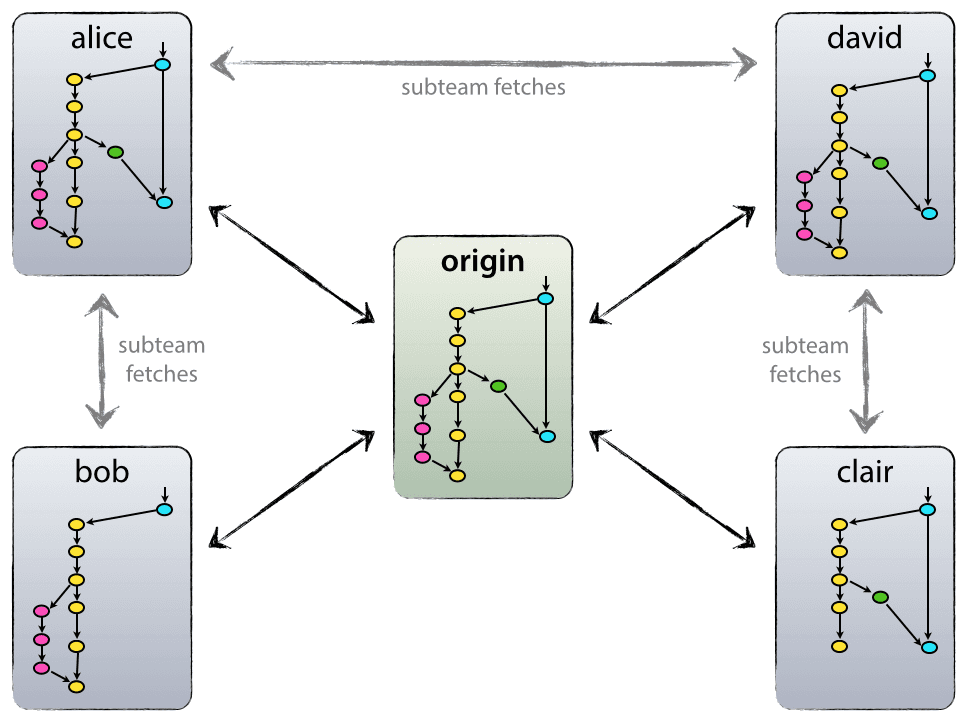
\includegraphics[height=0.8\textheight]{decentr}
    \end{figure}
\end{frame}

\begin{frame}
    \frametitle{Преимущества}
    \begin{itemize}
        \pause
        \item Локальные изменения
        \pause
        \item Отказоустойчивость
        \pause
        \item Довольный Линус
    \end{itemize}
\end{frame}

\begin{frame}
    \frametitle{Довольный Линус}
    \begin{figure}
        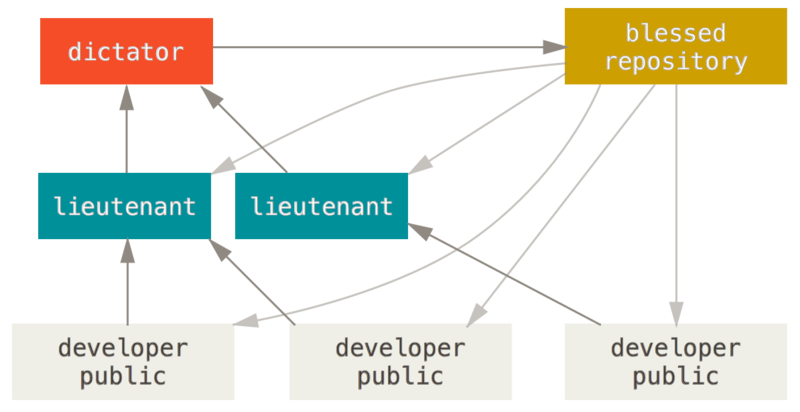
\includegraphics[width=\textwidth]{dictator}
    \end{figure}
\end{frame}

\section{Основные команды}

\begin{frame}[fragile]
    \frametitle{Самый бесполезный раздел}
    \pause
    \center
    \only<+>{
\includegraphics[height=0.8\textheight,keepaspectratio]{assistant.jpg}}
    \onslide<+->
    \begin{Verbatim}[fontsize=\relsize{-3}]
$ git
usage: git [--version] [--help] [-C <path>] [-c <name>=<value>]
           [--exec-path[=<path>]] [--html-path] [--man-path] [--info-path]
           [-p | --paginate | -P | --no-pager] [--no-replace-objects] [--bare]
           [--git-dir=<path>] [--work-tree=<path>] [--namespace=<name>]
           <command> [<args>]

These are common Git commands used in various situations:

start a working area (see also: git help tutorial)
   clone     Clone a repository into a new directory
   init      Create an empty Git repository or reinitialize an existing one

work on the current change (see also: git help everyday)
   add       Add file contents to the index
   mv        Move or rename a file, a directory, or a symlink
   restore   Restore working tree files
   rm        Remove files from the working tree and from the index

examine the history and state (see also: git help revisions)
   bisect    Use binary search to find the commit that introduced a bug
   diff      Show changes between commits, commit and working tree, etc
   grep      Print lines matching a pattern
   log       Show commit logs
   show      Show various types of objects
   status    Show the working tree status
    \end{Verbatim}
\end{frame}

\subsection{Начало работы}

\begin{frame}
    \frametitle{Установка}
    \onslide<1->\mintinline{bash}{$ sudo apt install git} \\
    \onslide<1->\mintinline{bash}{$ git config}
    \onslide<3->\mintinline{bash}{ --help}\\
    \onslide<4->\mintinline{bash}{$ man git-config}
    \onslide<2->
    \begin{exampleblock}{Пример}
        \mintinline{bash}{$ git config --global user.name "Artem Ohanjanyan"}
        \mintinline{bash}{$ git config --global user.email artemohanjanyan@gmail.com}
        \mintinline{bash}{$ git config --global core.editor vim}
    \end{exampleblock}
\end{frame}

\begin{frame}
    \frametitle{Получение репозитория}
    \begin{itemize}
        \item<2-> \mintinline{bash}{$ git init}
            \onslide<5->{\mintinline{bash}{ --help}}
        \item<3-> \mintinline{bash}{$ git clone}
            \onslide<5->{\mintinline{bash}{ --help}}
    \end{itemize}
    \onslide<4->
    \begin{exampleblock}{Пример}
        \mintinline{bash}{git clone https://github.com/artemohanjanyan/git-tutorial.git}
    \end{exampleblock}
\end{frame}

\subsection{Учёт изменений}

\begin{frame}
    \frametitle{Жизненный цикл файла}
    \center
    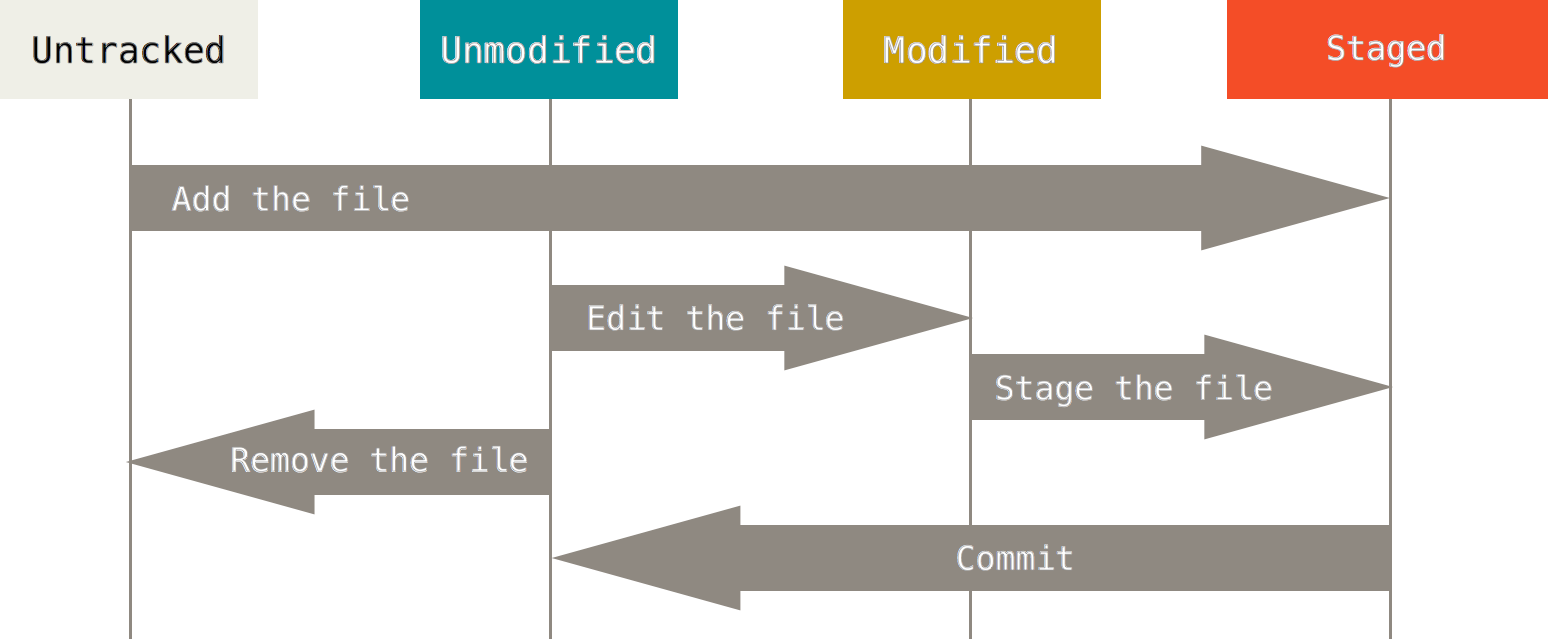
\includegraphics[width=0.9\textwidth]{lifecycle}
\end{frame}

\begin{frame}
    \frametitle{Команды}
    \begin{itemize}
        \item<1-> \mintinline{bash}{$ git add}
            \onslide<3->{\mintinline{bash}{ --help}}
        \item<1-> \mintinline{bash}{$ git mv}
            \onslide<3->{\mintinline{bash}{ --help}}
        \item<1-> \mintinline{bash}{$ git reset}
            \onslide<3->{\mintinline{bash}{ --help}}
        \item<1-> \mintinline{bash}{$ git rm}
            \onslide<3->{\mintinline{bash}{ --help}}
    \end{itemize}
    \onslide<2->
    \begin{exampleblock}{Пример}
        \mintinline{bash}{$ git add slides.tex}\\
        \mintinline{bash}{$ git mv dictator.png img/}
    \end{exampleblock}
\end{frame}

\subsection{Проверка}

\begin{frame}[fragile]
    \frametitle{Команды}
    \begin{itemize}
        \item<1-> \mintinline{bash}{$ git status}
            \onslide<3->{\mintinline{bash}{ --help}}
        \item<1-> \mintinline{bash}{$ git log}
            \onslide<3->{\mintinline{bash}{ --help}}
    \end{itemize}
    \onslide<2->
    \begin{exampleblock}{Пример}
        \begin{Verbatim}[fontsize=\relsize{-3},commandchars=\\\{\}]
$ git status
On branch bob
Changes to be committed:
  (use "git restore --staged <file>..." to unstage)
	\textcolor[HTML]{00aa00}{modified:   main.cpp}

Changes not staged for commit:
  (use "git add <file>..." to update what will be committed)
  (use "git restore <file>..." to discard changes in working directory)
	\textcolor[HTML]{aa0000}{modified:   main.cpp}

Untracked files:
  (use "git add <file>..." to include in what will be committed)
	\textcolor[HTML]{aa0000}{scoreboard}
        \end{Verbatim}
    \end{exampleblock}
\end{frame}

\begin{frame}[fragile]
    \frametitle{Команды}
    \begin{exampleblock}{Пример}
        \begin{Verbatim}[commandchars=\\\{\}]
$ git log --graph --decorate --oneline
*   \textcolor[HTML]{aa5500}{4d21842}\textcolor[HTML]{aa5500}{ (}\textcolor[HTML]{00aa00}{alice}\textcolor[HTML]{aa5500}{)} Merge branch 'bob' into alice
\textcolor[HTML]{aa0000}{|}\textcolor[HTML]{00aa00}{\textbackslash}
\textcolor[HTML]{aa0000}{|} * \textcolor[HTML]{aa5500}{f2af708}\textcolor[HTML]{aa5500}{ (}\textcolor[HTML]{00aaaa}{HEAD -> }\textcolor[HTML]{00aa00}{bob}\textcolor[HTML]{aa5500}{)} Add menu
\textcolor[HTML]{aa0000}{|} * \textcolor[HTML]{aa5500}{efbd2a5} Add score
* \textcolor[HTML]{00aa00}{|} \textcolor[HTML]{aa5500}{6ef17c4} Add Z-shapes
* \textcolor[HTML]{00aa00}{|} \textcolor[HTML]{aa5500}{6347d69} Add L-shapes
* \textcolor[HTML]{00aa00}{|} \textcolor[HTML]{aa5500}{b054512} Add line
\textcolor[HTML]{00aa00}{|}\textcolor[HTML]{00aa00}{/}
* \textcolor[HTML]{aa5500}{0d0461e} Add square
* \textcolor[HTML]{aa5500}{f4d5af4} Initial commit
        \end{Verbatim}
    \end{exampleblock}
\end{frame}

\subsection{Внесение изменений}
\begin{frame}
    \frametitle{Команды}
    \begin{itemize}
        \item<1-> \mintinline{bash}{$ git commit}
            \onslide<7->{\mintinline{bash}{ --help}}
        \item<2-> \mintinline{bash}{$ git checkout}
            \onslide<7->{\mintinline{bash}{ --help}}
        \item<3-> \mintinline{bash}{$ git diff}
            \onslide<7->{\mintinline{bash}{ --help}}
        \item<4-> \mintinline{bash}{$ git merge}
            \onslide<7->{\mintinline{bash}{ --help}}
        \item<5-> \mintinline{bash}{$ git branch}
            \onslide<7->{\mintinline{bash}{ --help}}
        \item<6-> \mintinline{bash}{$ git tag}
            \onslide<7->{\mintinline{bash}{ --help}}
    \end{itemize}
\end{frame}

\begin{frame}[fragile]
    \frametitle{git commit}
    \begin{block}{}
        \begin{minted}[fontsize=\footnotesize]{bash}
Commit message
# Please enter the commit message for your changes. Lines starting
# with '#' will be ignored, and an empty message aborts the commit.
#
# On branch bob
# Changes to be committed:
#	modified:   main.cpp
#
# Changes not staged for commit:
#	modified:   main.cpp
#
# Untracked files:
#	scoreboard
#
        \end{minted}
    \end{block}
\end{frame}

\begin{frame}
    \frametitle{git checkout}
    \center
    \begin{itemize}
        \pause
        \item \mintinline{bash}{$ git checkout master}
        \pause
        \item \mintinline{bash}{$ git checkout 6be2821}
        \pause
        \item \mintinline{bash}{$ git checkout -b feature}
    \end{itemize}
\end{frame}

\begin{frame}[fragile]
    \frametitle{git merge}
    \begin{itemize}
        \onslide<2->
        \item \mintinline{bash}{$ git merge feature}
        \onslide<3->
        \item merge-конфликты
        \onslide<5->
        \item fast-forward
    \end{itemize}
    \pause
    \onslide<4->
    \begin{exampleblock}{Пример}
        \begin{Verbatim}
<<<<<<< HEAD
Changes on master
=======
Changes on feature
>>>>>>> feature
        \end{Verbatim}
    \end{exampleblock}
\end{frame}

\subsection{Удалённые репозитории}
\begin{frame}[fragile]
    \frametitle{Удалённые ветки}
    \begin{Verbatim}[commandchars=\\\{\},fontsize=\relsize{-2}]
* \textcolor[HTML]{aa5500}{3d6c452}\textcolor[HTML]{aa5500}{ (}\textcolor[HTML]{aa0000}{upstream/master}\textcolor[HTML]{aa5500}{)} build version update 3.0.1
* \textcolor[HTML]{aa5500}{9d35a7a} Changelog updated for 3.0.1
* \textcolor[HTML]{aa5500}{425bd86} SolidMap equals improvement
*   \textcolor[HTML]{aa5500}{f96d7e1} Merge pull request #17 from artemohanjanyan/equals
\textcolor[HTML]{00aa00}{|}\textcolor[HTML]{aa5500}{\textbackslash}  
\textcolor[HTML]{00aa00}{|} * \textcolor[HTML]{aa5500}{670d71e}\textcolor[HTML]{aa5500}{ (}\textcolor[HTML]{aa0000}{origin/equals}\textcolor[HTML]{aa5500}{)} Add more tests
\textcolor[HTML]{00aa00}{|} * \textcolor[HTML]{aa5500}{ba53c22} Improve equals implementation
\textcolor[HTML]{00aa00}{|}\textcolor[HTML]{00aa00}{/}  
*   \textcolor[HTML]{aa5500}{b7bd7f3} Merge pull request #15 from artemohanjanyan/zipWith
\textcolor[HTML]{0000aa}{|}\textcolor[HTML]{E850A8}{\textbackslash}  
\textcolor[HTML]{0000aa}{|} * \textcolor[HTML]{aa5500}{7c55777} Generalize zipWith argument
\textcolor[HTML]{0000aa}{|} * \textcolor[HTML]{aa5500}{238c358} Add zipWith operator
* \textcolor[HTML]{E850A8}{|}   \textcolor[HTML]{aa5500}{d8c1109} Merge pull request #14 from artemohanjanyan/patch-1
\textcolor[HTML]{E850A8}{|}\textcolor[HTML]{aa0000}{\textbackslash} \textcolor[HTML]{E850A8}{\textbackslash}  
\textcolor[HTML]{E850A8}{|} \textcolor[HTML]{aa0000}{|}\textcolor[HTML]{E850A8}{/}  
\textcolor[HTML]{E850A8}{|}\textcolor[HTML]{E850A8}{/}\textcolor[HTML]{aa0000}{|}   
\textcolor[HTML]{E850A8}{|} * \textcolor[HTML]{aa5500}{72b251f} Update flatMap javadoc
\textcolor[HTML]{E850A8}{|}\textcolor[HTML]{E850A8}{/}  
* \textcolor[HTML]{aa5500}{652acad}\textcolor[HTML]{aa5500}{ (}\textcolor[HTML]{00aaaa}{HEAD}\textcolor[HTML]{aa5500}{ -> }\textcolor[HTML]{00aa00}{master}\textcolor[HTML]{aa5500}{, }\textcolor[HTML]{aa0000}{origin/master}\textcolor[HTML]{aa5500}{, }\textcolor[HTML]{aa0000}{origin/HEAD}\textcolor[HTML]{aa5500}{)} 3.0.0
    \end{Verbatim}
\end{frame}

\begin{frame}[fragile]
    \frametitle{Удалённые ветки}
    \begin{itemize}
        \item<1-3> \mintinline{bash}{$ git checkout -b equals origin/equals}
        \item<2-3> \mintinline{bash}{$ git checkout --track origin/equals}
        \item<3> \mintinline{bash}{$ git checkout equals}
    \end{itemize}
\end{frame}

\begin{frame}[fragile]
    \frametitle{Удалённые ветки}
    \begin{Verbatim}[commandchars=\\\{\},fontsize=\relsize{-2}]
* \textcolor[HTML]{aa5500}{3d6c452}\textcolor[HTML]{aa5500}{ (}\textcolor[HTML]{aa0000}{upstream/master}\textcolor[HTML]{aa5500}{)} build version update 3.0.1
* \textcolor[HTML]{aa5500}{9d35a7a} Changelog updated for 3.0.1
* \textcolor[HTML]{aa5500}{425bd86} SolidMap equals improvement
*   \textcolor[HTML]{aa5500}{f96d7e1} Merge pull request #17 from artemohanjanyan/equals
\textcolor[HTML]{00aa00}{|}\textcolor[HTML]{aa5500}{\textbackslash}  
\textcolor[HTML]{00aa00}{|} * \textcolor[HTML]{aa5500}{670d71e}\textcolor[HTML]{aa5500}{ (}\textcolor[HTML]{00aaaa}{HEAD}\textcolor[HTML]{aa5500}{ -> }\textcolor[HTML]{00aa00}{equals}\textcolor[HTML]{aa5500}{, }\textcolor[HTML]{aa0000}{origin/equals}\textcolor[HTML]{aa5500}{)} Add more tests
\textcolor[HTML]{00aa00}{|} * \textcolor[HTML]{aa5500}{ba53c22} Improve equals implementation
\textcolor[HTML]{00aa00}{|}\textcolor[HTML]{00aa00}{/}  
*   \textcolor[HTML]{aa5500}{b7bd7f3} Merge pull request #15 from artemohanjanyan/zipWith
\textcolor[HTML]{0000aa}{|}\textcolor[HTML]{E850A8}{\textbackslash}  
\textcolor[HTML]{0000aa}{|} * \textcolor[HTML]{aa5500}{7c55777} Generalize zipWith argument
\textcolor[HTML]{0000aa}{|} * \textcolor[HTML]{aa5500}{238c358} Add zipWith operator
* \textcolor[HTML]{E850A8}{|}   \textcolor[HTML]{aa5500}{d8c1109} Merge pull request #14 from artemohanjanyan/patch-1
\textcolor[HTML]{E850A8}{|}\textcolor[HTML]{aa0000}{\textbackslash} \textcolor[HTML]{E850A8}{\textbackslash}  
\textcolor[HTML]{E850A8}{|} \textcolor[HTML]{aa0000}{|}\textcolor[HTML]{E850A8}{/}  
\textcolor[HTML]{E850A8}{|}\textcolor[HTML]{E850A8}{/}\textcolor[HTML]{aa0000}{|}   
\textcolor[HTML]{E850A8}{|} * \textcolor[HTML]{aa5500}{72b251f} Update flatMap javadoc
\textcolor[HTML]{E850A8}{|}\textcolor[HTML]{E850A8}{/}  
* \textcolor[HTML]{aa5500}{652acad}\textcolor[HTML]{aa5500}{ (}\textcolor[HTML]{aa0000}{origin/master}\textcolor[HTML]{aa5500}{, }\textcolor[HTML]{aa0000}{origin/HEAD}\textcolor[HTML]{aa5500}{, }\textcolor[HTML]{00aa00}{master}\textcolor[HTML]{aa5500}{)} 3.0.0
    \end{Verbatim}
\end{frame}

\begin{frame}[fragile]
    \frametitle{Удалённые репозитории}
    \begin{itemize}
        \item<1-> \mintinline{bash}{$ git remote}
            \onslide<5->{\mintinline{bash}{ --help}}
        \item<2-> \mintinline{bash}{$ git fetch}
            \onslide<5->{\mintinline{bash}{ --help}}
        \item<3-> \mintinline{bash}{$ git push}
            \onslide<5->{\mintinline{bash}{ --help}}
        \item<4-> \mintinline{bash}{$ git pull}
            \onslide<5->{\mintinline{bash}{ --help}}
    \end{itemize}
    \begin{exampleblock}{Пример}
        \mintinline[fontsize=\relsize{-2}]{bash}{$ git remote add origin https://github.com/artemohanjanyan/git-tutorial.git}
    \end{exampleblock}
\end{frame}

\section{Советы}

\subsection{Коммиты}

\begin{frame}
    \frametitle{Коммиты}
    \pause
    \center
    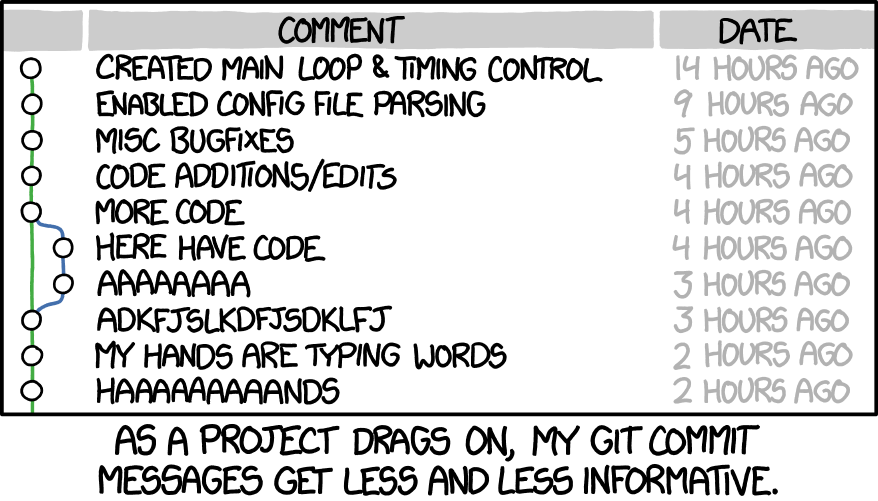
\includegraphics[width=0.95\textwidth]{commits}
\end{frame}

\begin{frame}
    \frametitle{Частота коммитов}
    \begin{itemize}
        \item Маленькие коммиты с конкретными изменениями
        \pause
        \item[$-$] \texttt{a lot of code}
        \pause
        \item[$-$] \texttt{something}
        \pause
        \item[$\pm$] \texttt{some progress on issue \#{}5}
        \pause
        \item[$+$] \texttt{Fix issue \#{}5}
    \end{itemize}
\end{frame}

\begin{frame}
    \frametitle{Сообщенния коммитов}
    \pause
    \begin{enumerate}
        \item Отделяем заголовок от тела пустой строкой.
        \item Заголовок не длиннее 50 символов,
        \item с большой буквы,
        \item без точки в конце,
        \item в повелительном наклонении.
        \item Тело умещаем в 72 символа по ширине,
        \item описываем в нём "<что">, а не "<как">.
    \end{enumerate}
\end{frame}

\begin{frame}[fragile]
    \frametitle{Пример}

    \newcommand{\sinceTwo}[1]{\onslide<3->{#1}}

    \pause
    \begin{Verbatim}[commandchars=\\\{\},fontsize=\relsize{-2}]
\sinceTwo{*   \textcolor[HTML]{aa5500}{5eab8ed} Merge pull request #6 from artemohanjanyan/master}
\sinceTwo{\textcolor[HTML]{00aa00}{|}\textcolor[HTML]{aa5500}{\textbackslash}  }
\sinceTwo{\textcolor[HTML]{00aa00}{|}} * \textcolor[HTML]{aa5500}{276da50} Compile pdf
\sinceTwo{\textcolor[HTML]{00aa00}{|}} * \textcolor[HTML]{aa5500}{611092f} Add \textbackslash{}mathrm to 'ord' keyword
\sinceTwo{\textcolor[HTML]{00aa00}{|}} * \textcolor[HTML]{aa5500}{0ba96ea} Use \textbackslash{}coloneqq instead of :=
\sinceTwo{\textcolor[HTML]{00aa00}{|}} * \textcolor[HTML]{aa5500}{6be881a} Use \textbackslash{}mathit for keywords such as 'Consis', 'Proof' etc
\sinceTwo{\textcolor[HTML]{00aa00}{|}} * \textcolor[HTML]{aa5500}{8cc97bb} Use function commands instead of plain names for better typesetting
\sinceTwo{\textcolor[HTML]{00aa00}{|}} * \textcolor[HTML]{aa5500}{85a128e} Use \textbackslash{}mid instead of | for better spacing
\sinceTwo{\textcolor[HTML]{00aa00}{|}} * \textcolor[HTML]{aa5500}{1d85a0c} Use \textbackslash{}with instead of \textbackslash{}& for better spacing
    \end{Verbatim}
\end{frame}

\subsection{Всякое}

\begin{frame}
    \frametitle{.gitignore}
    Перечисляем файлы, которые git должен игнорировать.
\end{frame}

\begin{frame}
    \frametitle{Ссылки на коммиты}
    \begin{itemize}
        \pause
        \item \texttt{HEAD}, \texttt{master}
        \pause
        \item \texttt{HEAD\~{}}
        \pause
        \item \texttt{HEAD\~{}\~{}\~{}}
        \pause
        \item \texttt{HEAD\~{}10}
        \pause
        \item \texttt{HEAD\^{}\^{}}
        \pause
        \item \mintinline{bash}{$ man git-rev-parse}
    \end{itemize}
\end{frame}

\begin{frame}
    \frametitle{SSH ключи}
    \begin{itemize}
        \item Чтобы не писать пароль каждый раз.
        \pause
        \item Создаём.
        \pause
        \item Открытый ключ отправляем на сервер.
        \pause
        \item Закрытым ключом доказываем, что мы это мы.
    \end{itemize}
\end{frame}

\begin{frame}
    \frametitle{Git flow}
    \pause
    \center
    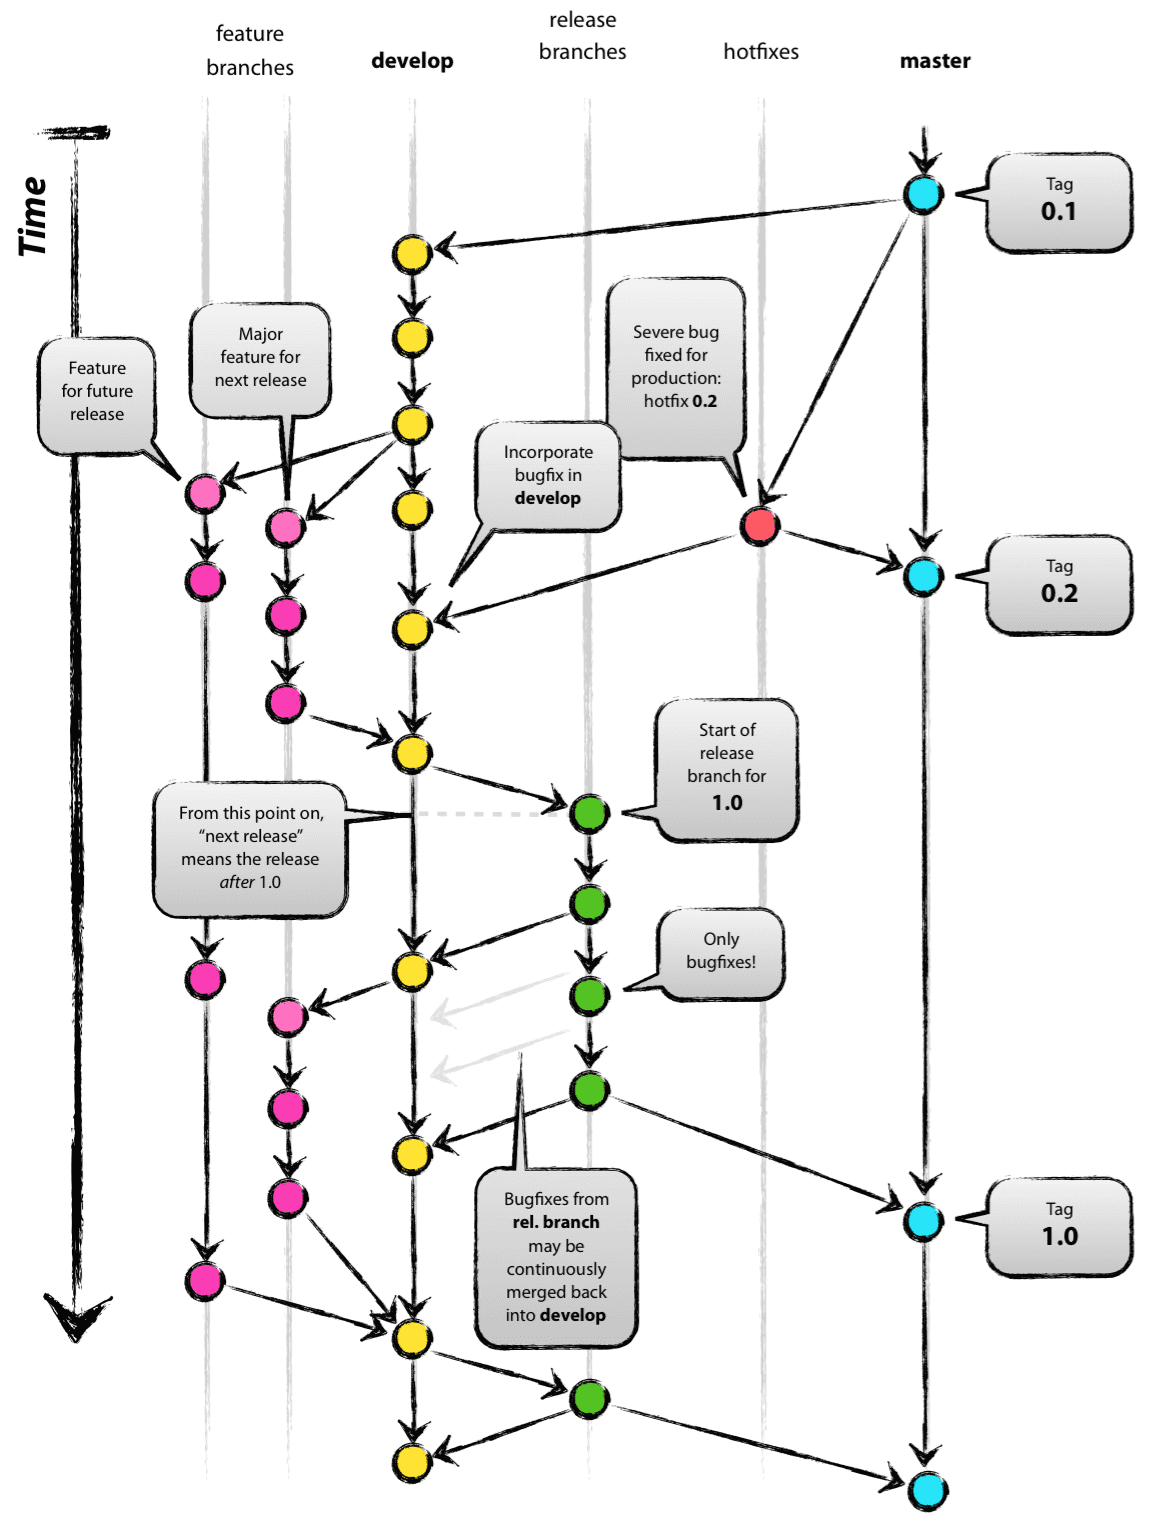
\includegraphics[height=0.8\textheight]{flow}
\end{frame}

\begin{frame}
    \frametitle{Danger zone}
    \begin{itemize}
        \item \mintinline{bash}{$ git rebase}
        \item \mintinline{bash}{$ git cherry-pick}
        \pause
        \item Опасно
        \pause
        \item \mintinline{bash}{$ git reflog}
        \item \mintinline{bash}{$ git reset}
    \end{itemize}
\end{frame}

\begin{frame}
    \frametitle{Альтернативы}
    \begin{itemize}
        \item Subversion "--- централизованная, старая.
        \item Mercurial "--- как git, но написана на Python.
    \end{itemize}
\end{frame}

\section{GitHub}

\begin{frame}
    \frametitle{Что такое GitHub?}
    \begin{itemize}
        \pause
        \item Бесплатные открытые репозитории
        \pause
        \item Pull request-ы
        \pause
        \item fork-и
        \pause
        \item \url{https://github.com/artemohanjanyan/git-tutorial}
            \pause\texttt{\#{}lol-2021}
    \end{itemize}
\end{frame}

\begin{frame}
    \frametitle{Альтернативы}
    \begin{itemize}
        \pause
        \item Bitbucket
        \pause
        \item GitLab
        \pause
        \item Gitea
    \end{itemize}
\end{frame}

\begin{frame}
    \frametitle{Ссылки}
    \url{https://www.google.com/}\\
    \url{https://git-scm.com/book}\\
    \url{https://github.com/artemohanjanyan/git-tutorial}\\
    \url{https://www.wix.engineering/post/virtual-monorepo-for-bazel}
\end{frame}

\begin{frame}
    \frametitle{Лекцию слушали}
    Илья, 8 класс, 2021. Спасибо за презентацию :)

\end{frame}

\begin{frame}
    \frametitle{Вопросы?}
    \pause
    Спасибо за внимание!
\end{frame}

\end{document}
